\documentclass[a4paper, oneside, uplatex, 12pt]{book}

\usepackage[backend=biber,style=ieee]{biblatex}
\usepackage[dvipdfmx]{graphicx}
\usepackage{latexsym}
\usepackage{bmpsize}
\usepackage{url}
\usepackage{comment}
\usepackage{hyperref}
\usepackage{nameref} % for in-doc references | \labal{} |  \ref{}  \nameref{}

\def\Underline{\setbox0\hbox\bgroup\let\\\endUnderline}
\def\endUnderline{\vphantom{y}\egroup\smash{\underline{\box0}}\\}

\newcommand{\ttt}[1]{\texttt{#1}}

%% bibliography
\addbibresource{./src/bibliography.bib}


\begin{document}

%% use roman page numbering for abstract and acknowledgements
\pagenumbering{roman}

% \title{\bf{\LARGE{Sample of \LaTeX  Document} \\ \Large{\LaTeX のサンプルコード}}}
% \author{木幡咲希\\早稲田大学}
% \date{28年28月28日(Tsu)}
% \maketitle

\begin{titlepage}
\begin{center}
    \vspace{0.1\textheight}
    {\Large Undergraduate Thesis 2023} \\
    \vspace{0.05\textheight}
    % 
\includegraphics[width=48truemm]{resources/0_title/waseda_logo.png} \\
    \vspace{0.05\textheight}
    \textbf{\huge TITLE!!!!!!!!!!!!!!!!!!!!!!!} \\
    \vfill
    {\Large Supervisor \hspace{0.02\textwidth} Edgar Simo-Serra} \\
    {\Large Area of Study \hspace{0.02\textwidth} Computer Graphics} \\
    \vspace{0.05\textheight}
    {\Large 
        Waseda University \\
        School of Fundamental Science and Engineering \\
        Department of Computer Science and Engineering \\}
    \vspace{0.05\textheight}
    {\Large 1W192140-3 Saki Kohata \\}
    \vspace{0.05\textheight}
    {Submitted on January.XX, 2023}
\end{center}
\end{titlepage}
    

%% abstract
\pagebreak
\hspace{0pt}
\vfill % magic commands to vertically center the content
    \begin{center}
    Abstract
    \end{center}
space for abstraction
\vfill
\pagebreak

%% acknowledgement
\pagebreak
\hspace{0pt}
\vfill 
    \begin{center}
    Acknowledgements
    \end{center}
    space for acknowledgements

\vfill
\pagebreak

%% use normal page numbering for the main body
\pagenumbering{arabic}

%% table of contents 
\tableofcontents
\listoffigures 
\listoftables

%% main body
\clearpage
\chapter{Introduction}
\section{Aim and Motivation} 
 This work makes the attempt to explore a path towards creating artificial
agents that can play the game of Pokemon on competitive levels through
methods of deep reinforcement learning. 

There are several motivations behind this goal. First of all, reinforcement
    learning(RL) has proposed a extremely powerful paradigm to create
    artificial intelligence, especially when paired with the representation
    power of deep neural networks. Since AlphaGO beat the human
    world champion in the game of Go in 2016, which is considered before to be
    impossible before by many scholars, RL is becoming increasingly active and
    promising as a research area. Some researchers even argues that the
    framework of RL is enough for intelligence of arbitrary complexity to arise
    in a recent publication . The reality is, despite the
    promises, that RL methods often suffer to perform or requires painfully
    time-consuming hyperparameter tuning in any task that is not a perfect
    information video game. This thesis, in the large picture, attempts to help
    closing the gap between theoretical promise and applicable reality of RL. 

This work also has an aspect of exploring possible solutions to 2 player
    imperfect-information games. Games are goal-oriented models of the real
    world, e.g. chess models a battle between two armies with different pieces
    representing different roles that exist in the real world.  The ideas
    represented by chess pieces are rather abstract, but human beings usually
    have no problem understanding the abstraction.  Recently, with the
    advancement of computer graphics, modern video games can now create almost
    photo-realistic gaming experience that, arguably, rivals the real world
    experience in complexity and intensity. Both classic board games and modern
    video games are goal-oriented and almost all of them can be played on a
    computer, which makes them the perfect test ground for artificial
    intelligence. Imperfect information games that require long term
    strategies, is one category of games that is much less studies compared to
    its perfect-information counterpart. Studying how imperfect-information
    games can be solved, using the case of Pokemon, records to be the second
    motivation of this thesis.
    
And last but certainly not least, as a long time Pokemon player myself, I
personally hold strong romantic values in the idea of creating something that
is better than myself in the game I love. The topic of the thesis is decided to
be such for the reasons discuss.


\section{Overview}
This thesis consist of 6 chapters, including this introduction chapter.
 pre explains some lower level building block
technologies used in this work including what is reinforcement learning, what
is a neural network and such. Chapter 3  introduces a selection
of recent researches including some state-of-the-art that this work took
inspiration from. Chapter 4explains the proposed methodologies
followed by Chapter which details the exact experiment setup
and presents the results. Finally in we will draw high
level conclusions of the whole thesis.


\chapter{Background}
\section{Machine Learning}

 Machine learning is a method of analyzing data in which a 
computer automatically iterates through large amounts of data 
without explicit programming to find patterns hidden in the data. 
The purpose of machine learning is to improve computer performance 
on a specific task over time through learning from data.
In other words, machine learning allows computers to adapt 
and improve performance on their own. 
Machine learning algorithms can be classified into two main 
categories: supervised learning and unsupervised learning. 

In Supervised learning, a model is trained on a labeled dataset,
which consists of input and corresponding output data. The model 
learns a function which maps the input data to the output data.
Once the model has learned this function, it can be used to make
predictions on unseen data, also known as out-of-sample data, 
that was not part of the original training dataset.
As an example, consider the task of predicting survival on the 
Titanic: the "Titanic - Machine Learning from Disaster" 
competition hosted by Kaggle\cite{titanic} requires participants 
to develop a model that accurately predicts whether an each person
on board survived the Titanic disaster or not. 
The model should be developed using the data in the training set.
The training set consists of information such as the gender and 
passenger ship class of each passenger on board and the results of 
whether the passenger survived or not.
The training set includes information about each passenger, such 
as their gender, age and ship class, and the outcome of whether 
they survived or not. This labeled data is used to build a machine
learning model that can predict whether they survived  based on 
other available information of the passengers.

In contrast to supervised learning models, which rely on labeled 
training data, unsupervised learning models do not use such data.
Since the goal of unsupervised learning is to find unknown patterns
that exist in the data, we only provide the input data to the model.
The model discovers regularities and features on its own, without
the guidance of labeled training data.

\begin{figure}[h]
  \centering
  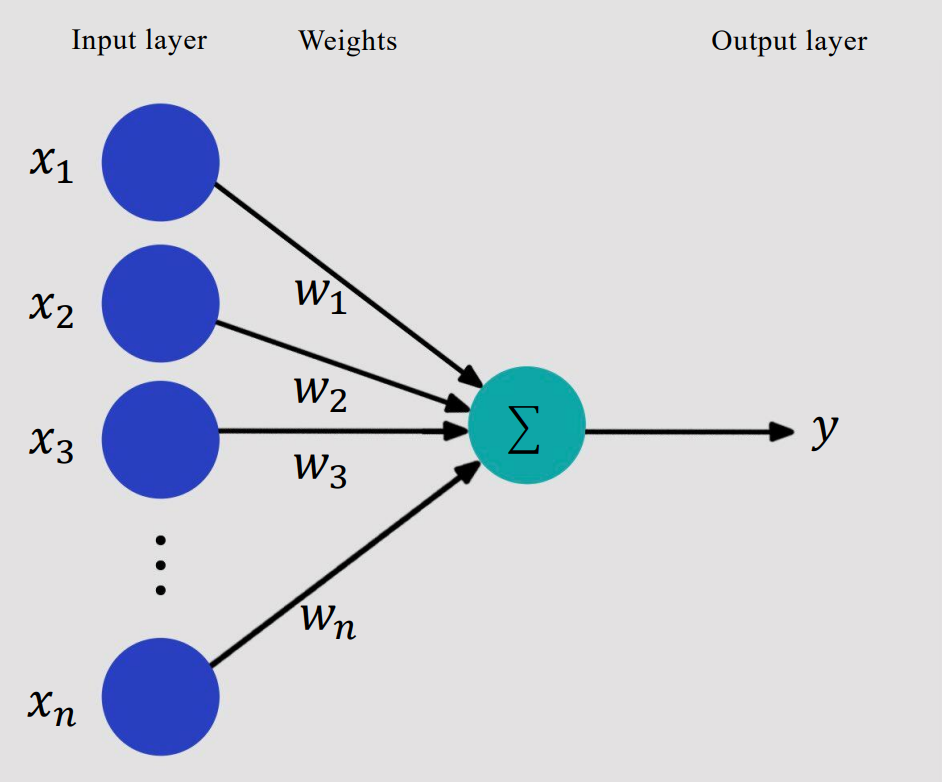
\includegraphics[width=130truemm]{resources/2_background/simple_perceptron.png}
  \caption{
    An example of simple perceptron
  }
  \label{simple_perceptron}
\end{figure}

\section{Neural Networks}
 Neural networks are a kind of machine learning algorithms which 
algorithm is modeled after the function and structure of human 
neural circuits and consist of a large number of interconnected 
processing nodes called neurons.
Frank Rosenblatt's simple perceptron \cite{Rosenblatt1958ThePA} was 
an early example of an artificial neural network. 
Simple perceptron consists of a single neuron that receives inputs 
from multiple sources and generates a single output. 
The structure of it is shown in Figure \ref{simple_perceptron}. 
The figure clearly shows how the perceptron processes received inputs.
The inputs $x_1, x_2 ... x_n$ are multiplied by their respective weights
$w_1, w_2 ... w_n$ and summed to produce the output $y$.
This can be expressed mathematically as follows:
\begin{equation}
  \label{perceptron_output}
  y = \sum_{k}w_k x_k + b
\end{equation}
where $b$ is a term called bias which is a variable that determines 
whether or not the output $y$ is set to 1.
During simple perceptron training, the goal is to find the optimal 
weights $w_1, w_2 ... w_n$, that will produce the correct output for 
a given set of inputs.
However, simple perceptrons are limited in its learning ability because 
they can only model linear relationships between inputs and outputs.
Therefore more complex neural networks are needed for learning tasks 
that require the modeling of nonlinear relationships.
A multilayer perceptron, which is a multilayer version of a simple 
perceptron, is one example. Figure \ref{multilayer_perceptron} shows
the most basic multilayer perceptron, which consists of three layers: 
an input layer, a hidden layer, and an output layer.

\begin{figure}[h]
  \centering
  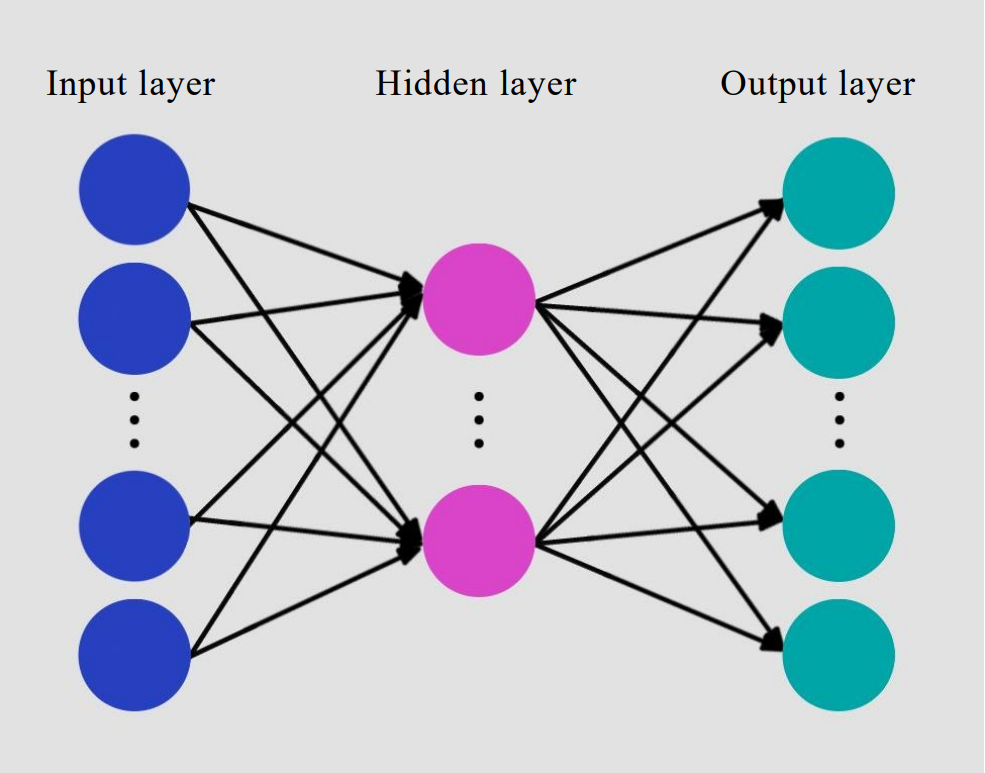
\includegraphics[width=130truemm]{resources/2_background/multi_layer_perceptron.png}
  \caption{
    An example of multi layer perceptron
  }
  \label{multilayer_perceptron}
\end{figure}

これで非線形問題が解ける理由を簡単に書く。隠れ層を2対上にしたものもMLP。
多層パーセプトロンよりも隠れ層を増やせば、より複雑な関数が表現できるのでは?
で、ディープラーニングの導入。

\cite{dastres:hal-03349542}

\section{Deep Learning}
隠れ層を増やしたニューラルネットワーク。層が"深い"からDeep Learning。
ディープラーニングネットワークの画像。(これはあくまで基本形)
活性化関数につなげる方法が難しい~
【やっぱ活性化関数について単純パーセプトロンか多層パーセプトロンのとこで
説明するべきだったか。。。】

\section{Convolutional Neural Network}
画像データを対象とする場合に用いる。(通常のNNでも画像は適用できるが、
要素を縦一列にしないといけない。画像は縦横の位置情報が重要。一列に
してしまっては重要なデータが失われる。二次元のまま利用できるのが理想)
で、うまれたのがCNN。画像を二次元のまま入力に用いることができる。

畳み込みとかプーリング、全結合とかはここで説明する。

\section{Transformers}
あああああああああああ

\section{まだ何か必要だと思う} 
ああああああああああああ
\chapter{Related Works}

\section{Image Style Transfer}
 Gatys \textit{et al}. \cite{Gatys_2016_CVPR} introduced \textit{A Neural Algorithm 
of Artistic Style} which enables the creation of novel images that seamlessly blend 
the subject matter of a photograph with the artistic style of a famous artwork.
In rendering the semantic content of an image in various styles, the problem was
the lack of effective image representations that can explicitly encode semantic 
information and separate image content and style. 
\textit{A Neural Algorithm of Artistic Style} \cite{Gatys_2016_CVPR} is able to 
analyze the visual characteristics of an image and separate them into two distinct 
components: the content and the style.
The content refers to the subject or object depicted in the image, while the style 
refers to the visual techniques manifested in a painting, such as touch and mood.

The algorithm in the paper uses a convolutional neural network (CNN) to extract
content and style features from two input images. The goal is to generate an 
output image that minimizes the difference between the content and style features 
of the input and output images, as measured by two loss functions defined in the 
paper. 

To minimize the difference in content features between the input and output images,
it is necessary to consider reducing the content loss function. 
Let $\vec{p}$ and $\vec{x}$ be the input image and the image that is generated by
the model, and  $P^l$ and $F^l$ be their feature representations of these images in 
layer l of the CNN. Then the loss function of the content of images is defined as:

\begin{equation}
    \label{contentloss}
    \mathcal{ L}_{content}(\vec{p}, \vec{x}, l)=\frac{1}{2} \sum_{i, j}\left(F_{i j}^l-P_{i j}^l\right)^2
\end{equation}
Similarly, to minimize the difference in style features between the input and
output images, we consider reducing the style loss function. The style of an 
image can be represented by the correlations of the outputs of the filters in 
each layer. This feature correlation is given by a Gram matrix, which is 
expressed as:
\begin{equation}
    G_{i j}^l = \sum_k F_{i k}^l F_{j k}^l 
\end{equation}
Let $\vec{a}$ and $\vec{x}$ be the input image and the image that is generated by
the model, and $A^l$ and $G^l$ be their style representations of these images in 
kayer l of the CNN. The contribution of layer l to the total loss can be 
expressed as:
\begin{equation}
    E_l=\frac{1}{4 N_l^2 M_l^2} \sum_{i, j}\left(G_{i j}^l-A_{i j}^l\right)^2
\end{equation}
Based on this, we can define the loss function for the style of images as:
\begin{equation}
    \label{styleloss}
    \mathcal{ L}_{style}(\vec{a}, \vec{x})=\sum_{l=0}^\mathcal{ L}w_{l}E_{l}
\end{equation}
To transfer the style of image $\vec{a}$ to image $\vec{p}$, it is needed to 
create a new image that maintains the content representation of $\vec{p}$ 
while adopting the style representation of $\vec{a}$. To achieve this, we must 
minimize both Equation \ref{contentloss} and Equations \ref{styleloss}.
The final loss function to minimize is:

\begin{equation}
    \mathcal{ L}_{total}(\vec{p}, \vec{a}, \vec{x})=\alpha\mathcal{ L}_{content}(\vec{p}, \vec{x})+\beta\mathcal{ L}_{style}(\vec{a}, \vec{x})
\end{equation}


Figure \ref{output_IST} shows the images generated using this algorithm.
絵の出所の説明。

筆のタッチなどのスタイルが適応されていて、良い結果だと思う。が、色味や
特徴的なオブジェクトのトランスファーが行われてしまっている。
私が取り組むものではそれはやりたくない。

\begin{figure}
    \centering
    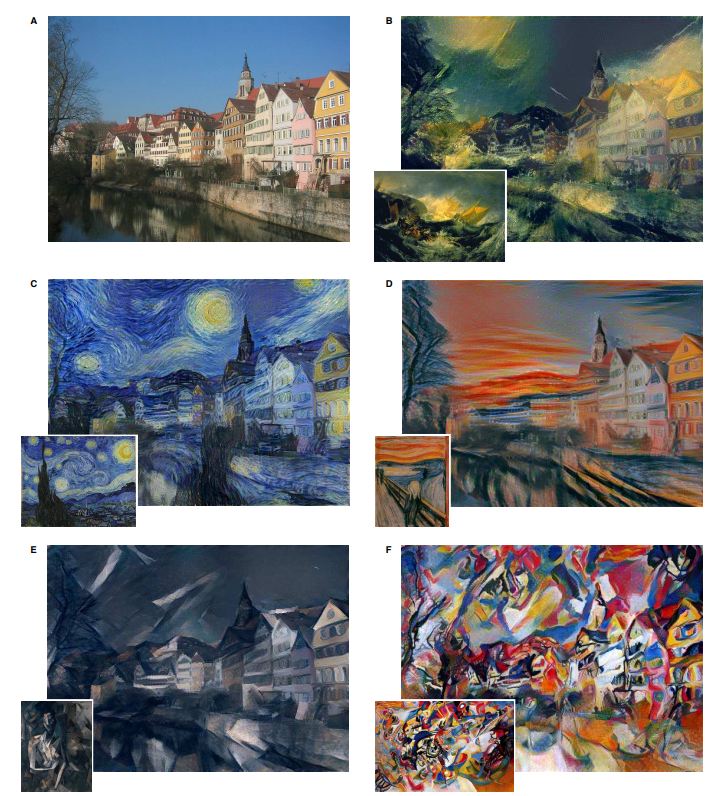
\includegraphics[width=150truemm]{resources/3_related_work/outputs_IST.png}
    \caption{
      なにかかく. Figure taken from
      \cite{Gatys_2016_CVPR}. 
    }
    \label{output_IST}
\end{figure}


\section{強化学習版}
Learn to paint \cite{Huang_2019_ICCV}
\section{Learn to PaintのCNN版}
Paint Transformers \cite{liu2021paint}

その論文にて課題として残っている点は何であるか、自分の研究はそれとはどのように異なるか、という点が明確になるように
\chapter{Methodology}
Danさん, 林さん, zhenさん, Yuanさん, BachelorThesisが参考になりそう。
\section{Loss Function}

ブラシの形状を決めるときのロス関数
\chapter{Experiments and Results}


\chapter{Discussions}

\section{Future Work} 
 In this study, we utilized a Transformer-based framework called Paint 
Transformer \cite{liu2021paint} for transforming the content of the input image 
to match the brush style of a reference image.
Our model used the Paint Transformer as is, to train a stroke prediction model, 
and therefore, the brush parameters were the same as the original, including 5 
shape parameters and 3 color parameters. However, we believe that adding more 
parameters could make the stroke expression more flexible in future works.
Accordingly, it is also necessary to rethink the loss function for brush style 
comparisons.

In the model we introduced in this paper, each stroke in the painting is created 
by simply adjusting the size of the brush image, as shown in Figure \ref{strokeparams}.
However, there is another technique that can be used to create brushstrokes 
- repeating the same brush image multiple times in succession.
For example, in a painting software Clip Studio \cite{clipstudio}, it is 
possible to draw strokes like in Figure \ref{goodstroke}.
\begin{figure}[h]
    \centering
    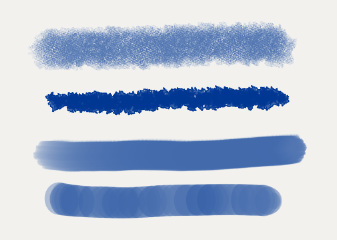
\includegraphics[width=63truemm]{resources/6_discussions/strokes-clipstudio.png}
    \caption{
        Strokes drawn in Clip Studio.
    }
    \label{goodstroke}
\end{figure}
\newline
These types of strokes cannot be created simply by extending the base brush 
image. Although these strokes are created by various settings such as repeating 
pattern, spacing between the repetition, and strength of brush entry and exit, 
it would be possible to increase the expression of the strokes with just 
expressing the strokes as the simple repetition of the base brush image.
For example, using brush (e) and (f) in Figure \ref{Brushes} as the base brush, the 
generated brush stroke shown in Figure \ref{results} is unnatural, and this is 
believed to be because the strokes are represented by scaling the base image. 
If the expressiveness of the brush is increased, believed that the model generate 
strokes like in the Figure \ref{stroke-shouldbe}. As a result, it is expected 
that more natural images can be generated. 
Additionally, in the original stroke expression, the color is monochrome, 
but it is expected that the expressiveness will increase by making it possible 
to express the gradation.

\begin{figure}[h]
    \centering
    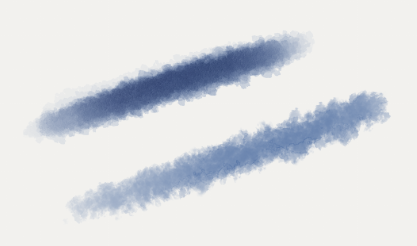
\includegraphics[width=100truemm]{resources/6_discussions/coral_cloud.png}
    \caption{
        Strokes that would be depicted by brushes (e) and (f) in Figure \ref{Brushes},
        drawn in Clip Studio.
    }
    \label{stroke-shouldbe}
\end{figure}


By increasing the brush parameters, it is expected that the stroke expression 
can be made more flexible and the result picture generated by the model will 
be better.
Furthermore, various extensions such as the ability to draw curved strokes and 
consideration for blending color of strokes can also be considered in addition 
to the above discussion.

\section{Conclusion}
 In this research, we introduced a novel approach that utilizes FNNs to 
transform the content of the input image to match the brush style of a 
reference image.
To achieve this, we prepared multiple brush images used to generate the strokes.
Our ultimate goal is to produce strokes that closely emulate the brush style of 
the reference image, however, our current research is still far from achieving 
this goal due to the inflexibility of the strokes, including the small number 
of stroke parameters. There is still room for improvement in the way strokes 
are expressed, and it is expected that the accuracy of mimicking brush style 
will improve with these improvements.




% \section{はじめに}
% \begin{figure}[t]
%     \begin{center}
%         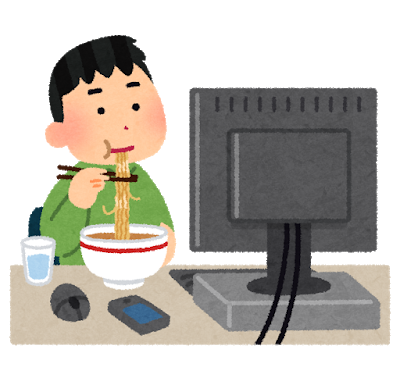
\includegraphics[width=7cm]{image/syokuji_computer.png}
%         \caption{パソコンの前でご飯を食べる人のイラスト}
%         \label{fig:syokuji_computer}
%     \end{center}
% \end{figure}

% パソコンの前でご飯を食べることはよくある。パソコンの前でご飯を食べる人のイラストを図\ref{fig:syokuji_computer}に示す。
% このイラストは、規約の範囲内であれば、個人、法人、商用、非商用問わず無料で利用できることでおなじみの、{\bf かわいいフリー素材 いらすとや}\cite{irasutoya}より引用した。
% \cite{liu2021paint}

% \section{おわりに}
% やっぱり{\bf いらすとや}のイラストはすばらしい。


%% bib
\printbibliography


\end{document}
